\newpage
\subsection{Caso d'uso UC5: Recupero password}
\label{UC5}
\begin{figure}[ht]
	\centering
	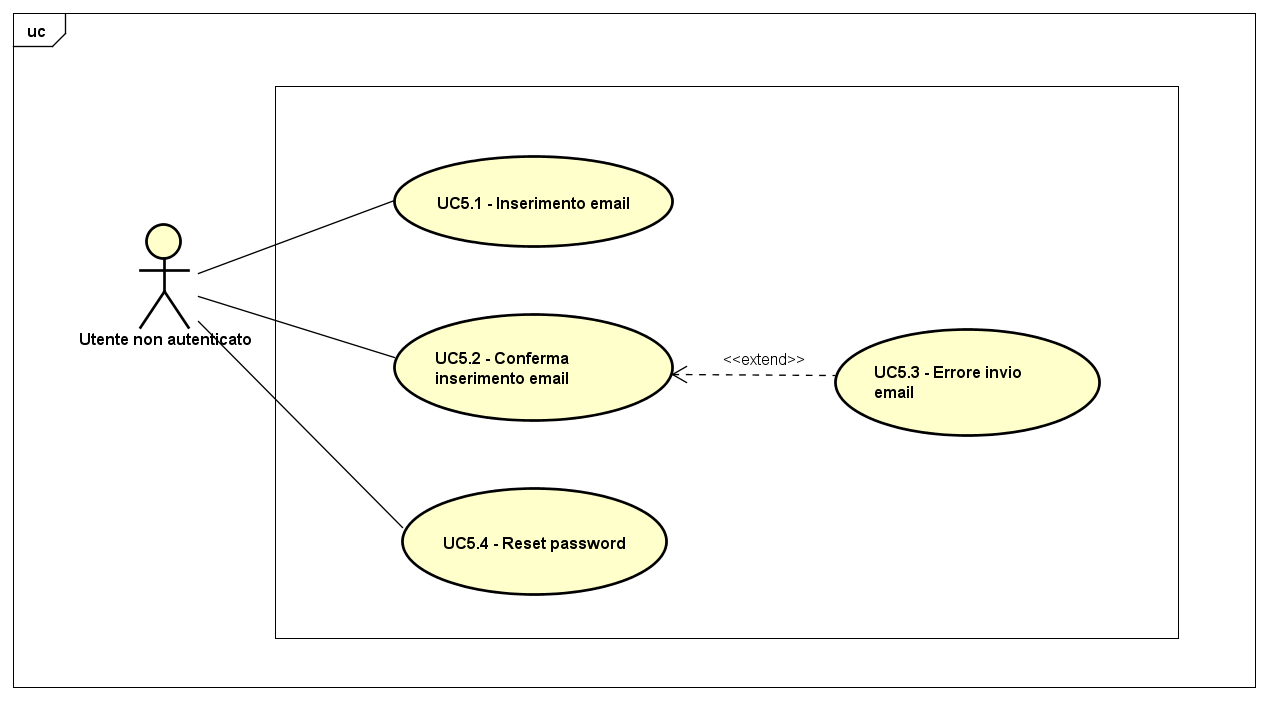
\includegraphics[scale=0.45]{UML/UC5.png}
	\caption{UC5: Recupero password}
\end{figure}

\begin{longtable}{ l | p{11cm}}
	\hline
	\rowcolor{Gray}
	 \multicolumn{2}{c}{UC5 - Recupero password} \\
	 \hline
	\textbf{Attori} & Utente non autenticato \\
	\textbf{Descrizione} & L'attore recupera la password del proprio account API Market tramite l'invio di una email \\
	\textbf{Pre-Condizioni} & L'attore ha scelto di recuperare la password del proprio account API Market \\
	\textbf{Post-Condizioni} & L'attore ha ricevuto nella propria casella email un link per resettare la password del proprio account API Market, oppure la procedura è fallita \\
	\textbf{Scenario Principale} & 
	\begin{enumerate*}[label=(\arabic*.),itemjoin={\newline}]
		\item L'attore può inserire la propria email (UC5.1)
		\item L'attore può confermare l'indirizzo email inserito, al quale l'applicazione web invierà un link per resettare la password (UC5.2)
	\end{enumerate*}\\
	\textbf{Scenari Alternativi} & 
	\begin{enumerate*}[label=(\arabic*.),itemjoin={\newline}]
		\item L'attore, se ha inserito un'email non valida o inesistente, può visualizzare un messaggio d'errore e l'email di reset password non viene inviata (UC5.3)
		\item L'attore, se ha richiesto il recupero della password ed ha aperto il link per poterla resettare, può effettuare il reset password in una apposita schermata (UC5.4)
	\end{enumerate*}\\
\end{longtable}